

\chapter{Introduction}
\label{chapter:introduction}

Exception handling~\cite{JavaException} attributes to the response of program during runtime to some
exceptional condition encounter. Most of the time it changes normal flow of
program. In many cases exception handling is natural part of software execution
due to the nature of the software.
An application which constantly accesses I/O which also includes share resources
may throw exception if another application blocks it.
Here in this paper we discuss and analyze java exceptions and produce repair
patch based on that. Java supports two types of exceptions :

\begin{itemize}
  
  \item \textbf{Checked exception} which requires explicit \emph{throws}
  declaration at the method declaration or \emph{try-catch} block by the
  developers. Such exceptions are handled carefully as they often involves
  accessing resources like network, database, file system, I/O etc.
  Code snippet~\ref{checkedexception} and~\ref{checkedexception1} is an example of a
  checked exception type when one needs to read userinput from the console.
  
  \item \textbf{Unchecked exception} which does not enforce similar handing
  mechanism as the former one.
  \emph{java.lang.RuntimeException}~\cite{RuntimeException} and its subclasses
  and \emph{java.lang.Error}~\cite{JavaError} are types of unchecked exceptions.
  \emph{NullPointerException}, \emph{ArrayIndexOutOfBound},
  \emph{ArithmeticException} are examples of common java runtime exceptions.
  Code snippet~\ref{uncheckedexception} is an eample where the method returns an
  integer after performing division operation. If the denominator is zero then
  this operation will throw an \emph{ArithmeticException} \emph{divide-by-zero}.
  But as arithmetic exception is a runtime exception and which is a unchecked
  exception, we do not need to write a throw keyword or put try-catch block.
  
\end{itemize}

\onehalfspacing
\lstset{language=Java, caption=Example 1 of java checked exception,
label=checkedexception}
\begin{lstlisting}
void foo() throws IOException
{
 InputStremReader is = new InputStremReader(System.in);
 BufferedReader br = new BufferedReader(is);
 String str = br.readline();
}
\end{lstlisting}


\lstset{language=Java, caption=Example 2 of java checked exception ,
label=checkedexception1}
\begin{lstlisting}
void foo()
{
 try
 {
  InputStremReader is = new InputStremReader(System.in);
  BufferedReader br = new BufferedReader(is);
  String str = br.readline();
 }
 catch(IOException ex)
 {
  System.err.println("IO Exception happend");
 }
}

\end{lstlisting}

\lstset{language=Java, caption=Example of java unchecked exception,
label=uncheckedexception}
\begin{lstlisting}
int foo(int a, int b)
{
 return a/b;
}
\end{lstlisting}

\doublespacing

Oracle official documentation says that ``\emph{Here's the bottom line
guideline: If a client can reasonably be expected to recover from an exception,
make it a checked exception. If a client cannot do anything to recover from the
exception, make it an unchecked exception}".
Unchecked exception, particularly runtime exceptions can be thrown from any
point in the program making them quite unpredictable in nature.
Due to this extensive testing phase is required to eliminate any bugs and solve
corner cases.
Yet many applications suffer unexpected runtime exception causing system crash
which leads to shutdown or restart.

We find out many applications where system shutdown/restart is expensive due to
their nature.

% \begin{figure}[!htb]
% \centering
% 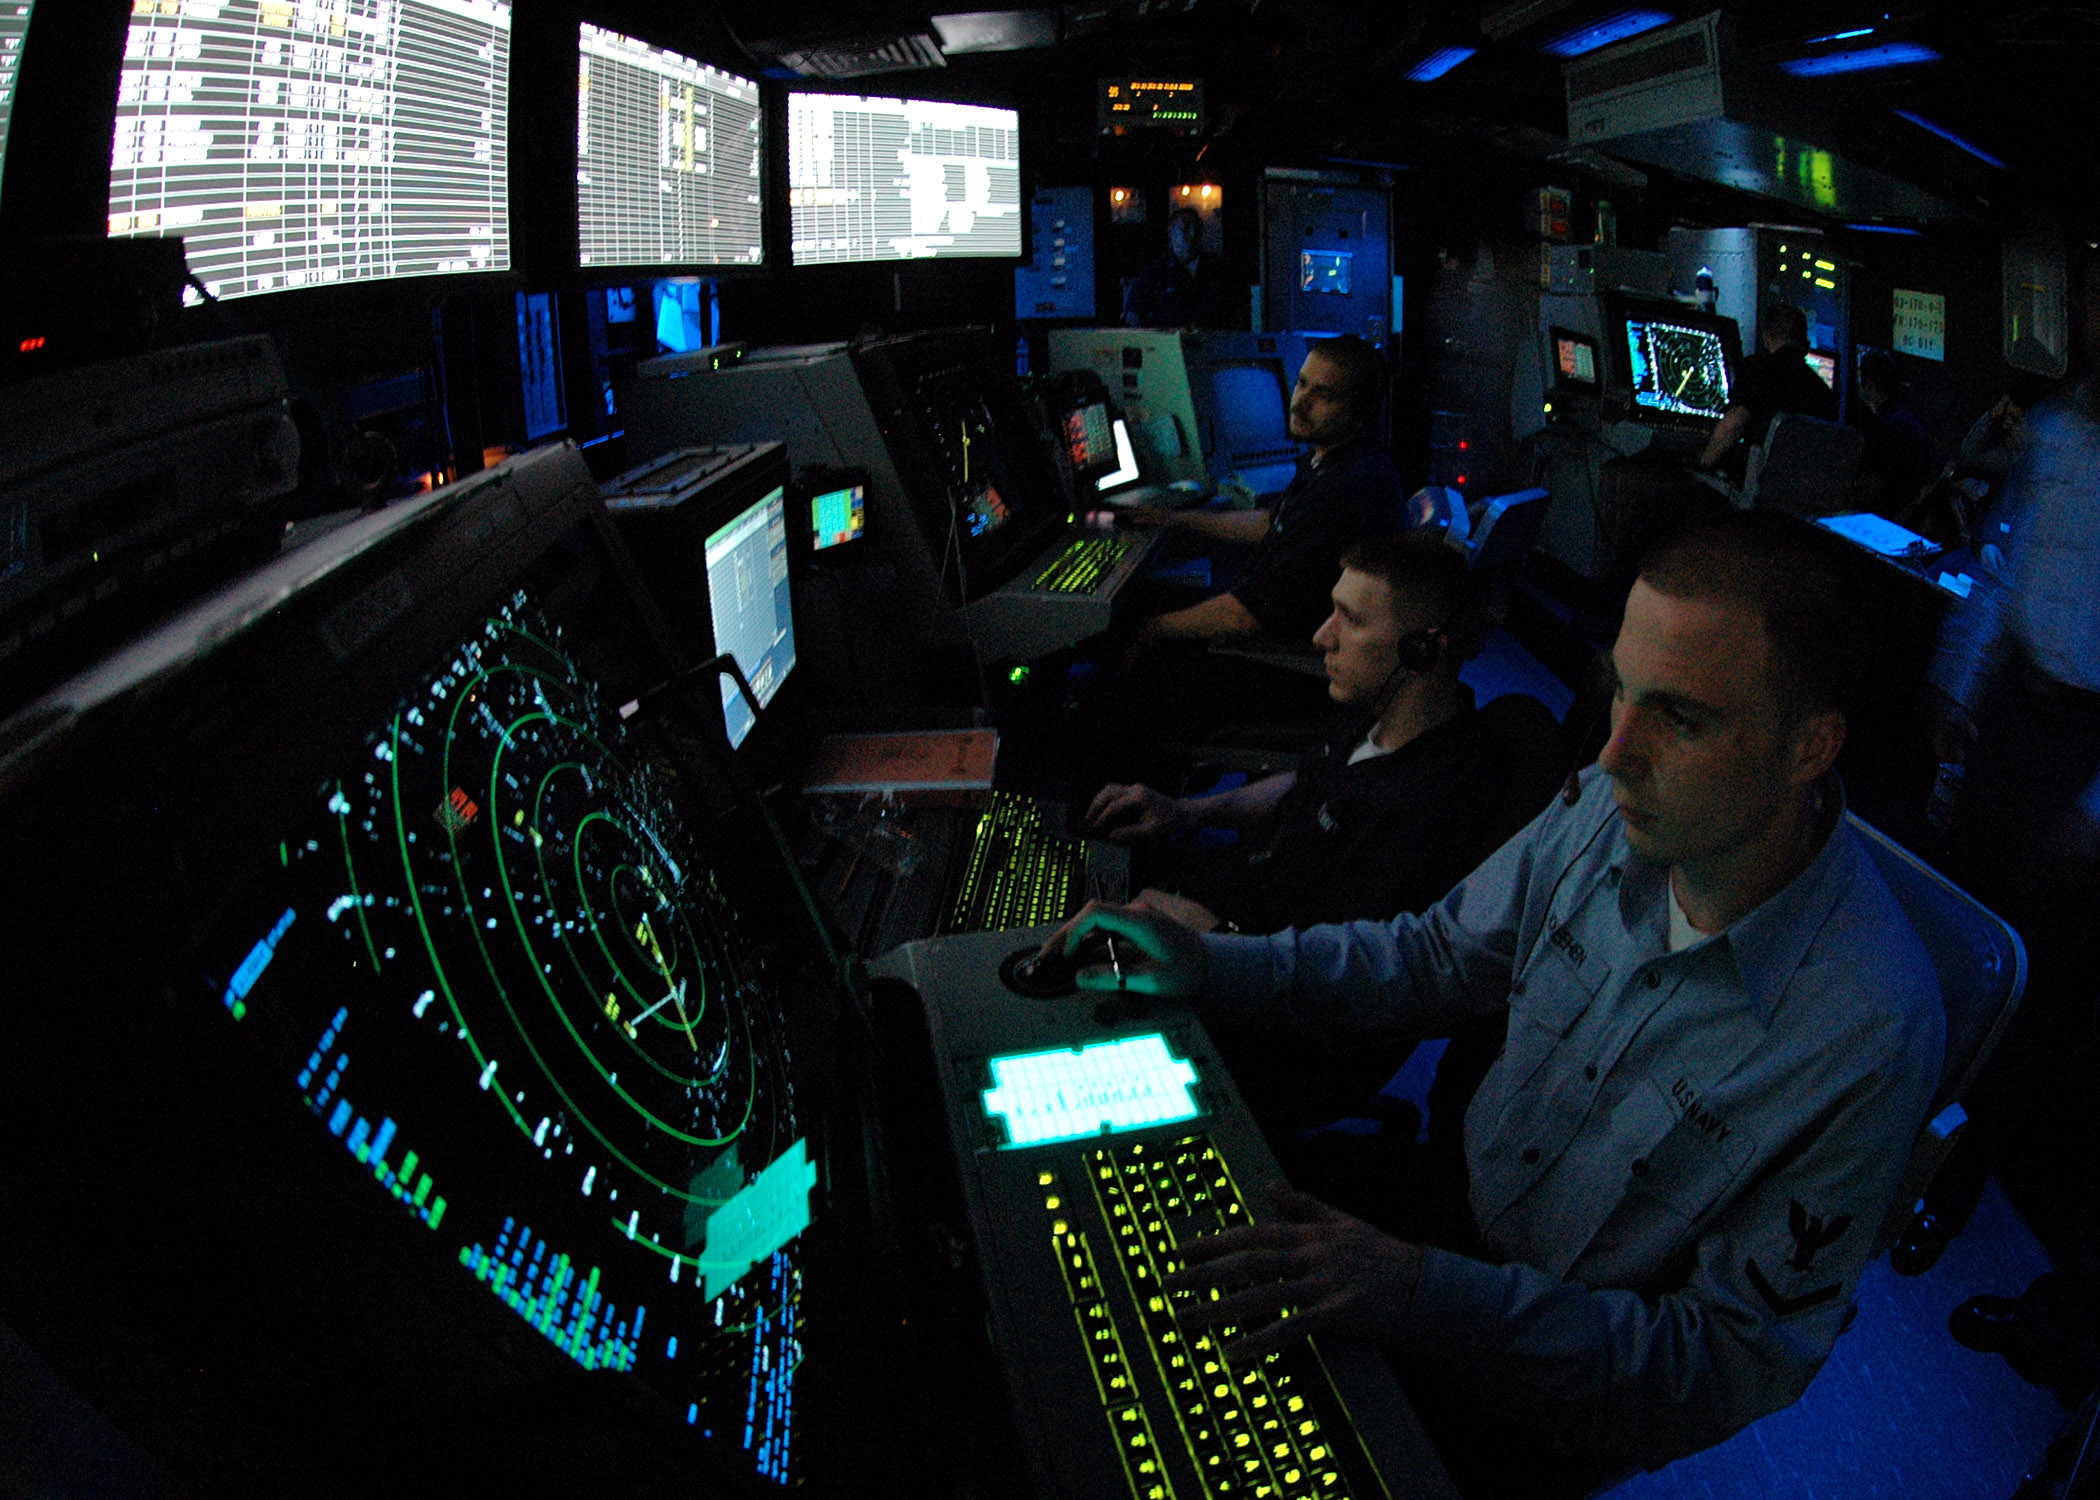
\includegraphics[width=3.3in]{images/ATC.jpg}
% \caption{Air Traffic Controller (ATC) which controls several airplanes
% simultaniously}
% \label{fig:atc}
% \end{figure}
% 
% \begin{tabular}{cc}
% \subfloat{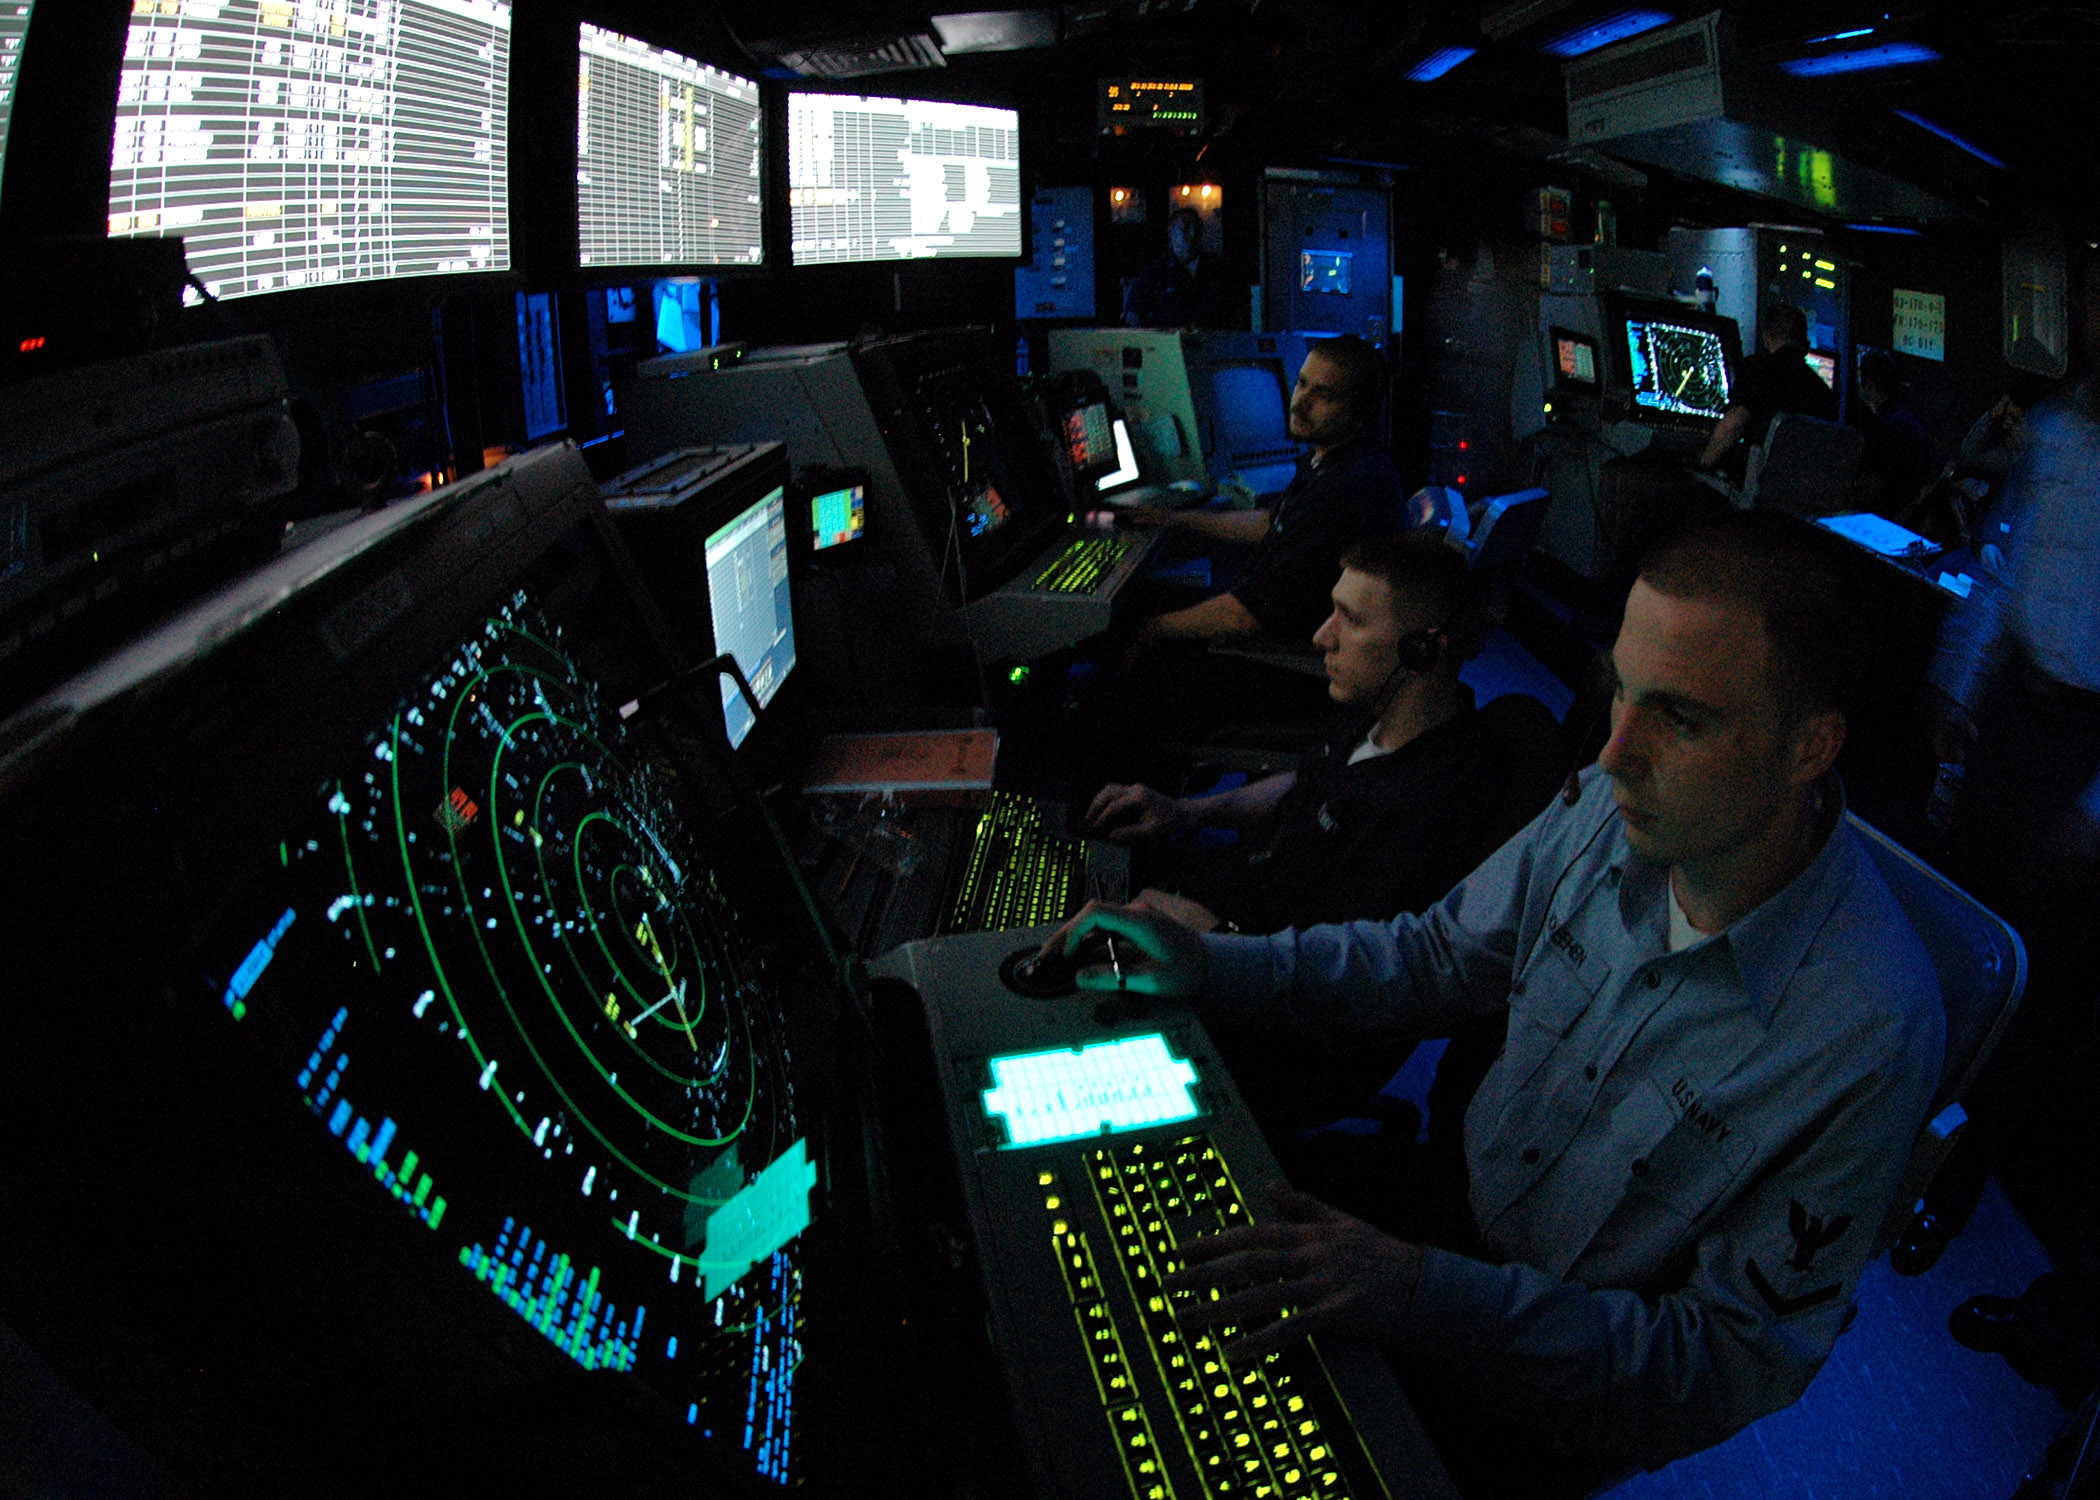
\includegraphics[width = 2in]{images/ATC.jpg}} &
% \subfloat{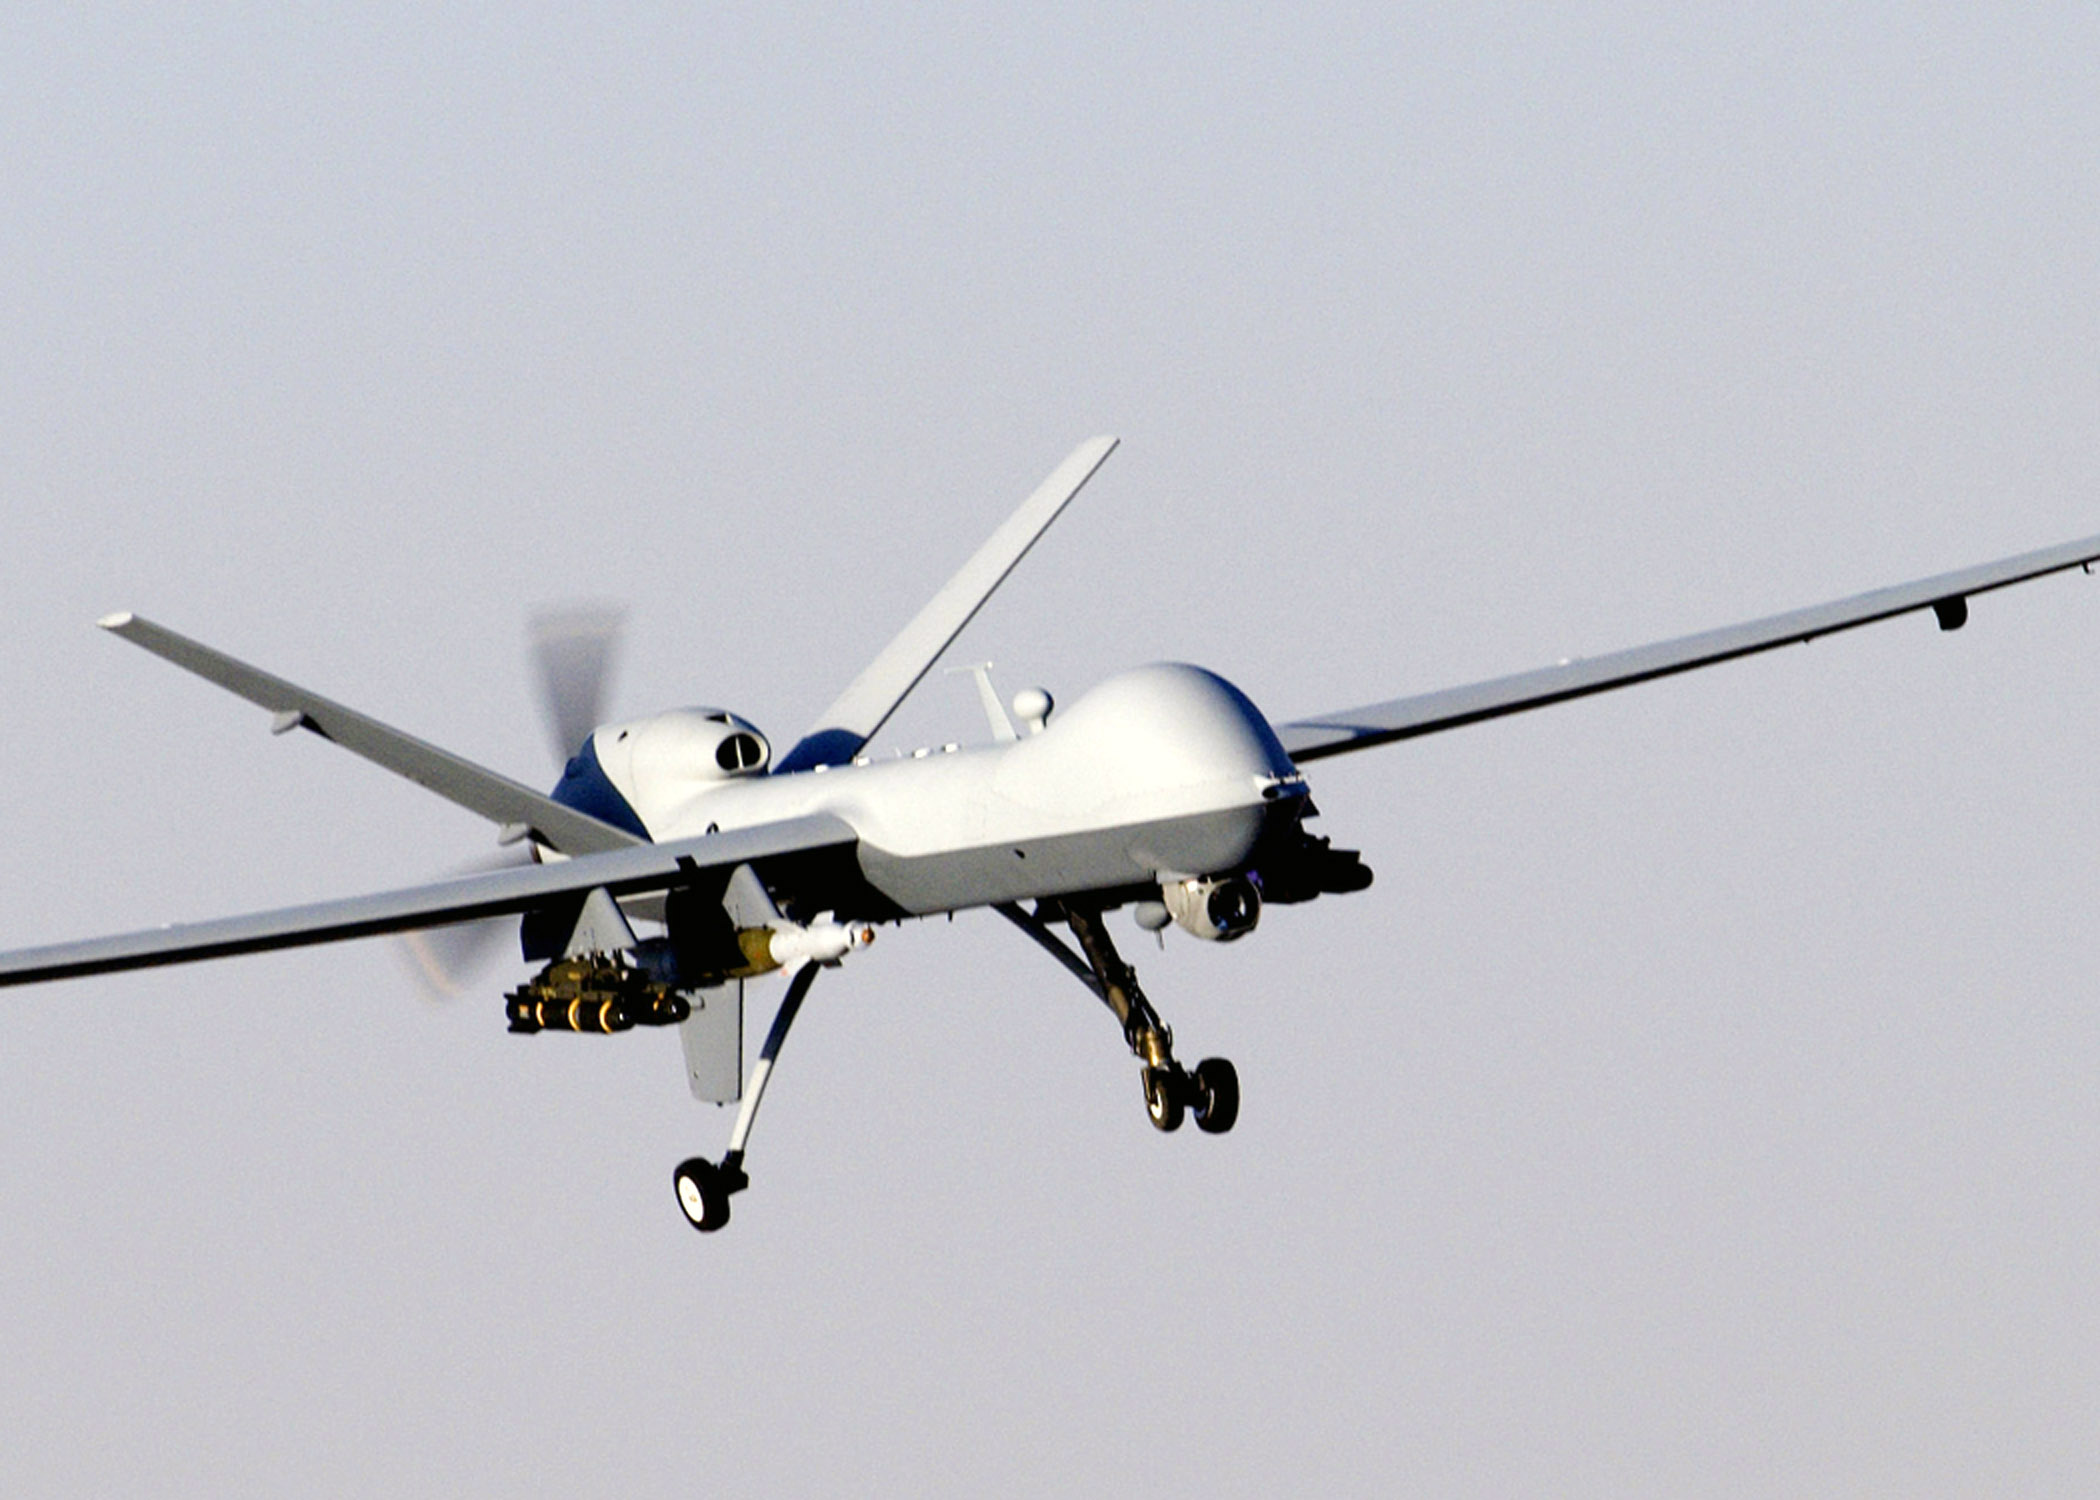
\includegraphics[width = 2in]{images/UAV.jpg}} \\
% \subfloat{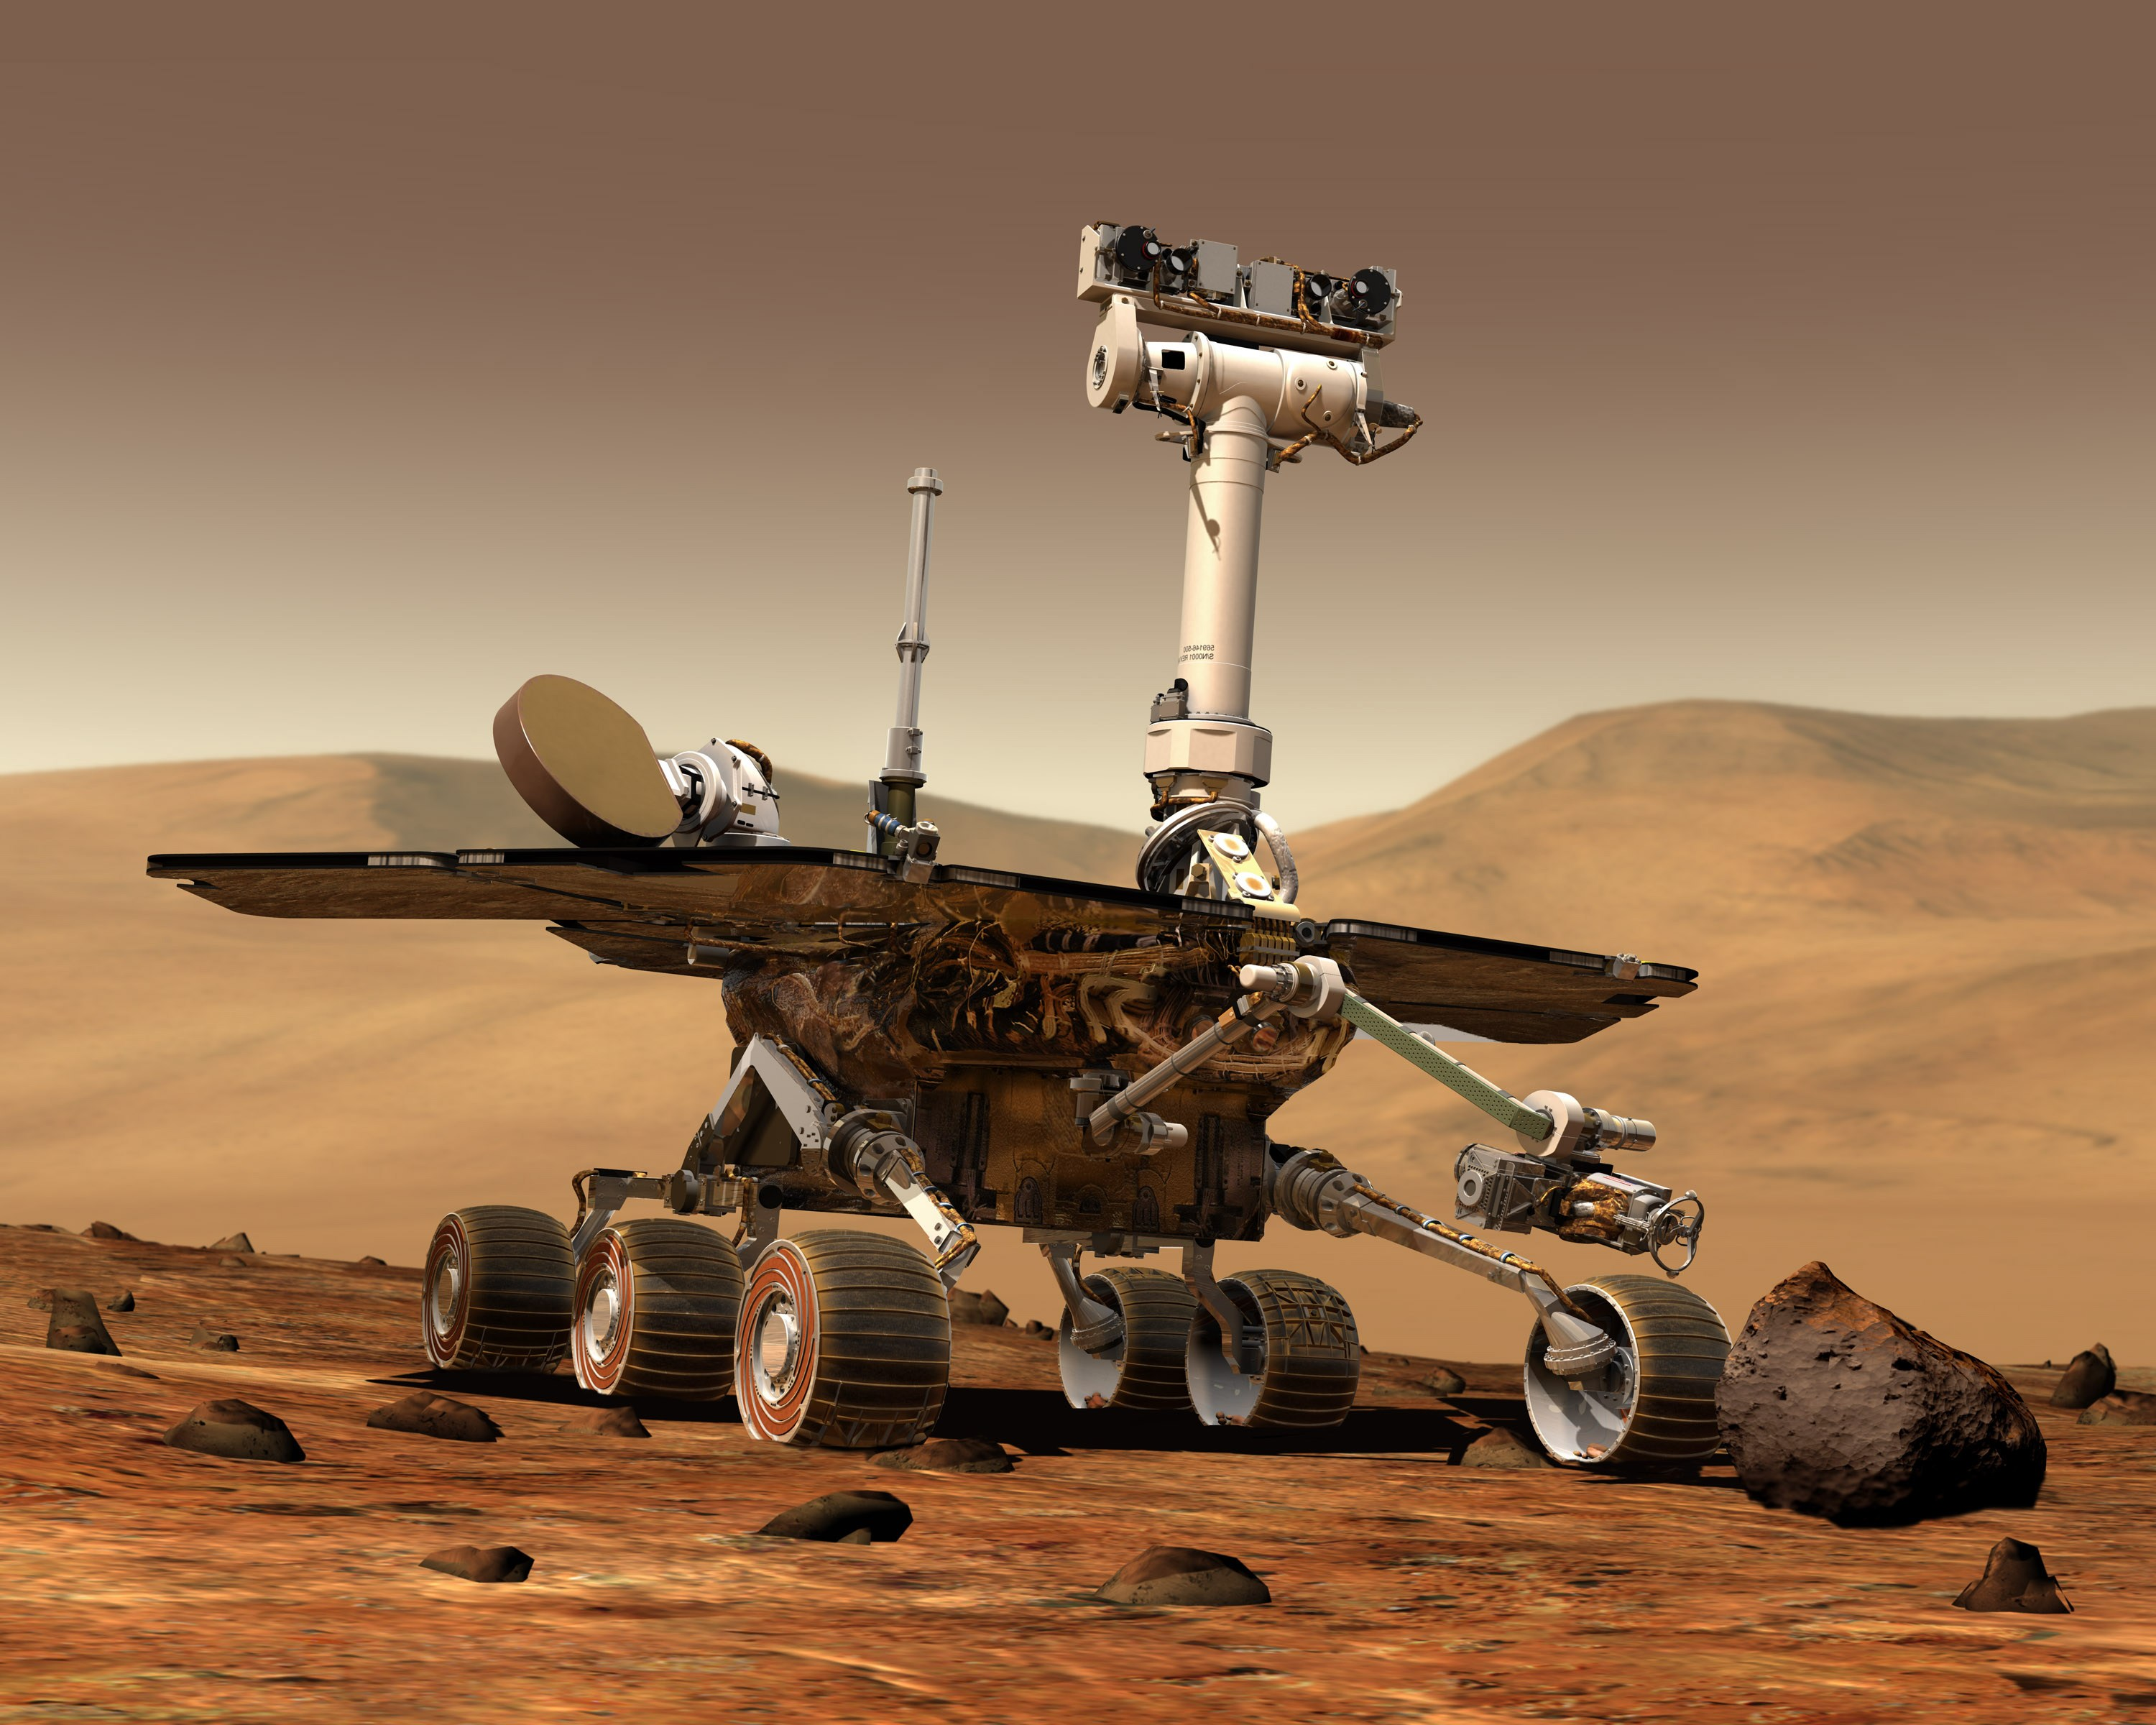
\includegraphics[width = 2in]{images/ROVER.jpg}} &
% \subfloat{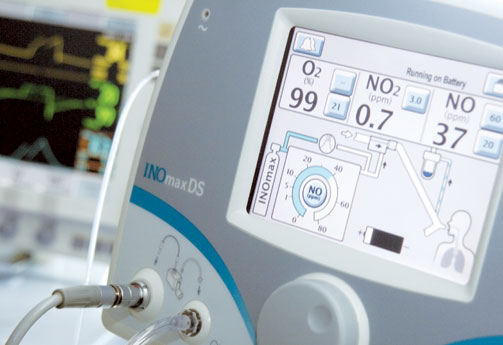
\includegraphics[width = 2in]{images/LSS.jpg}}
% \end{tabular}

\begin{figure}
\begin{subfigure}{.5\textwidth}
  \centering
  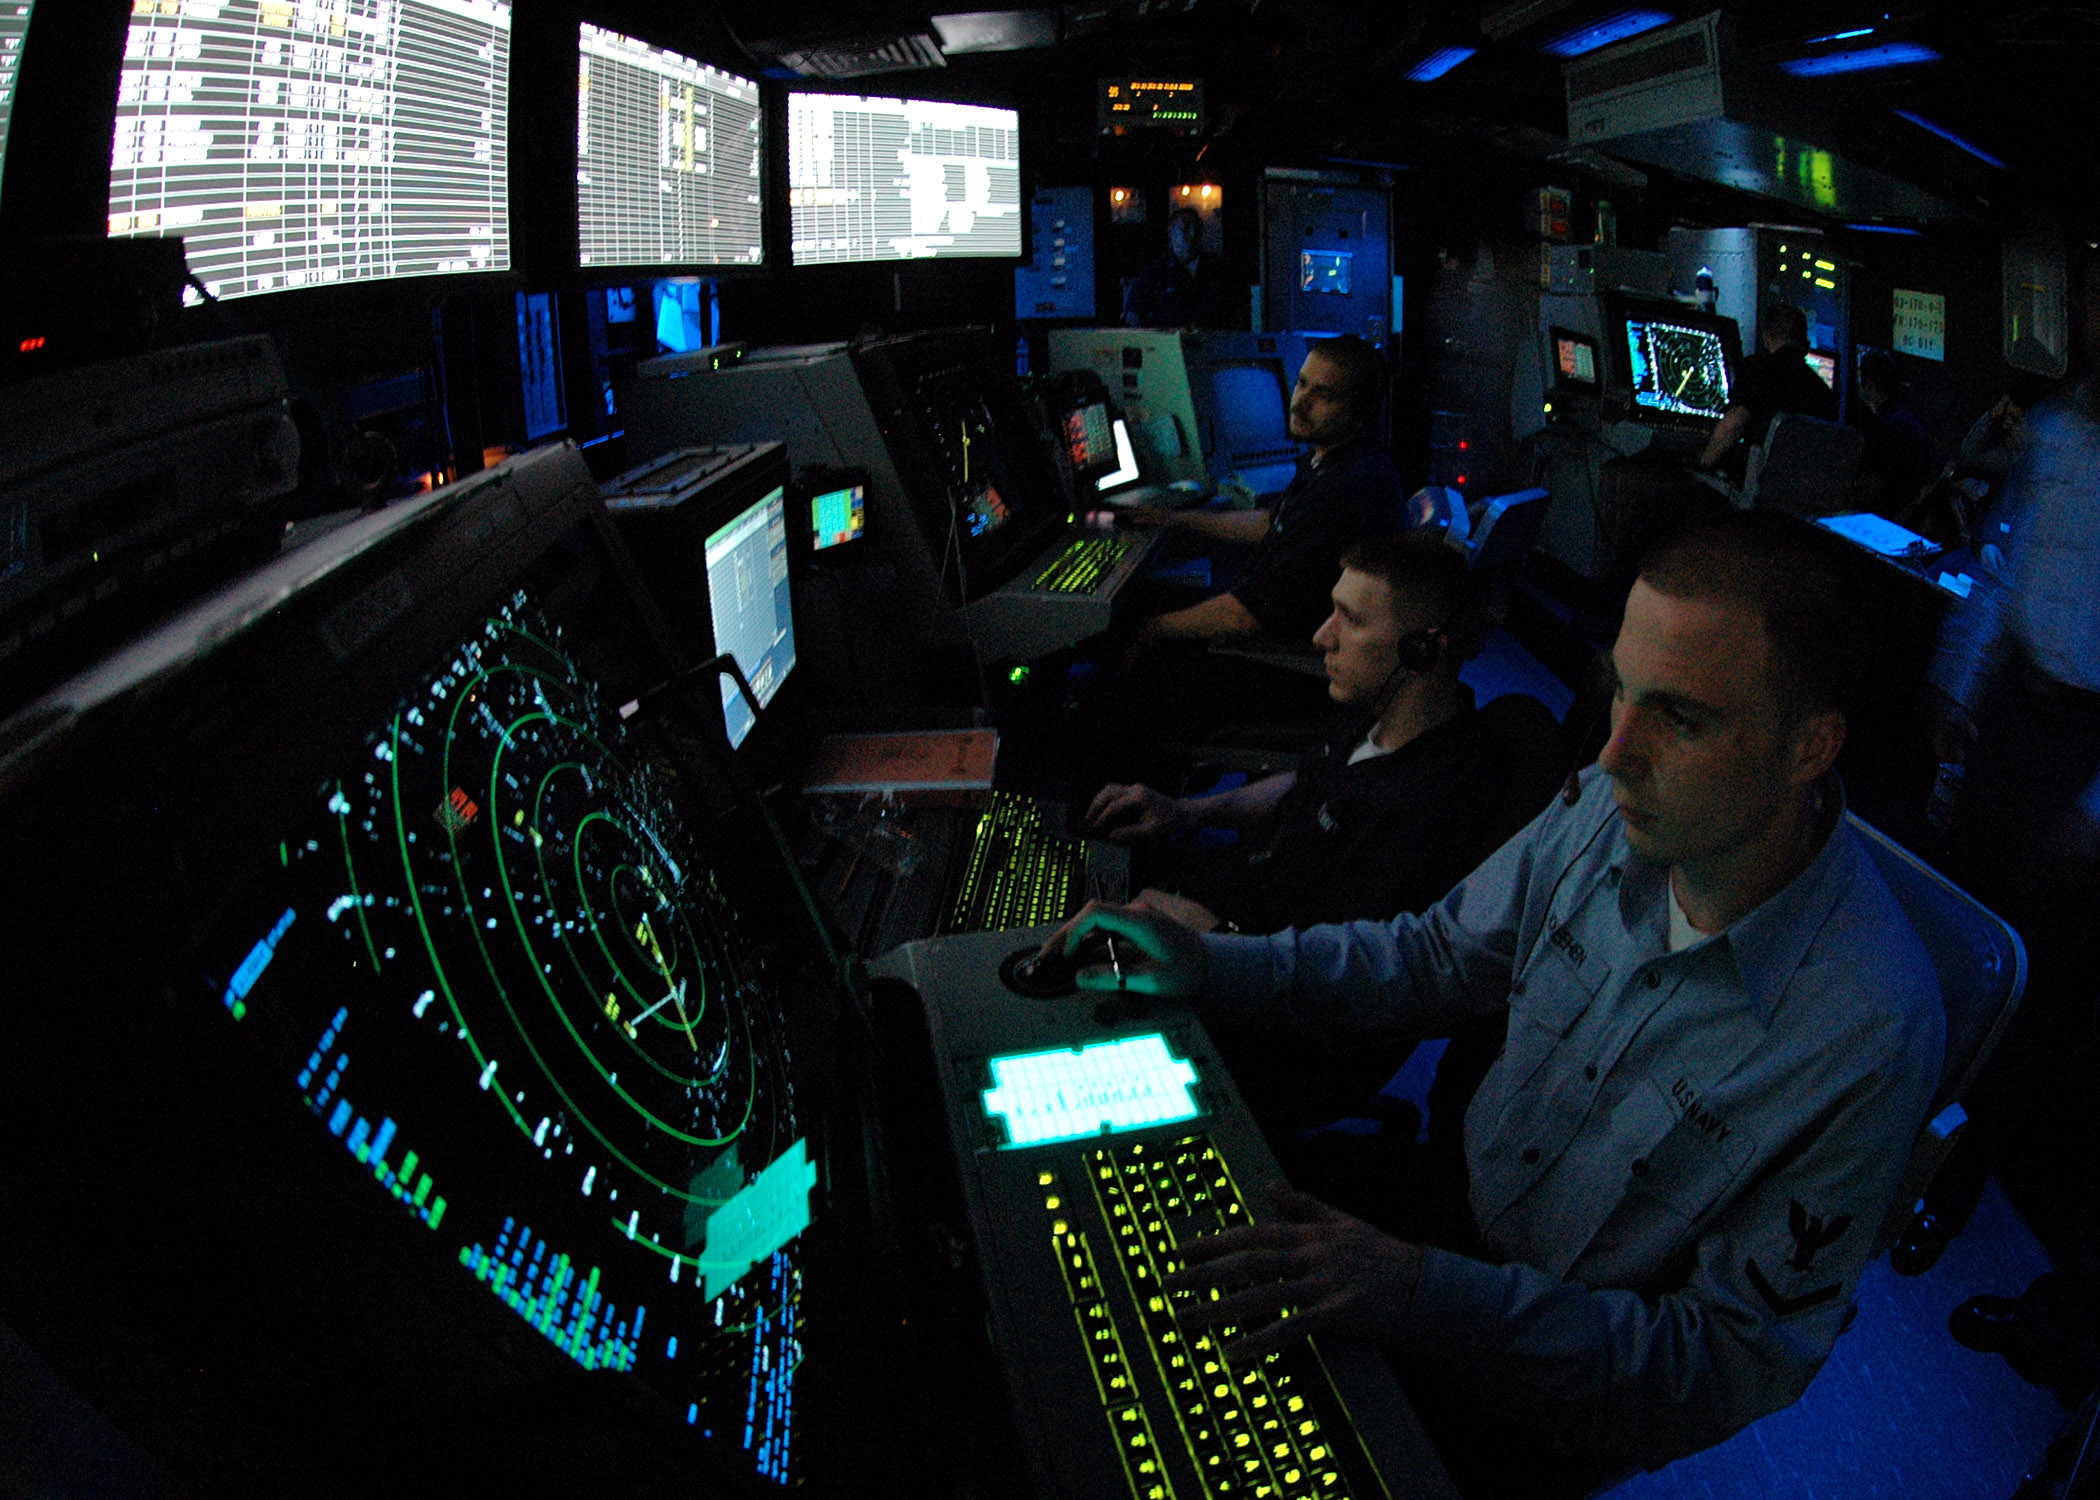
\includegraphics[width=.9\linewidth]{images/ATC.jpg}
  \caption{Air Traffic Controller (ATC)}
  \label{fig:sfigATC}
\end{subfigure} %
\begin{subfigure}{.5\textwidth}
  \centering
  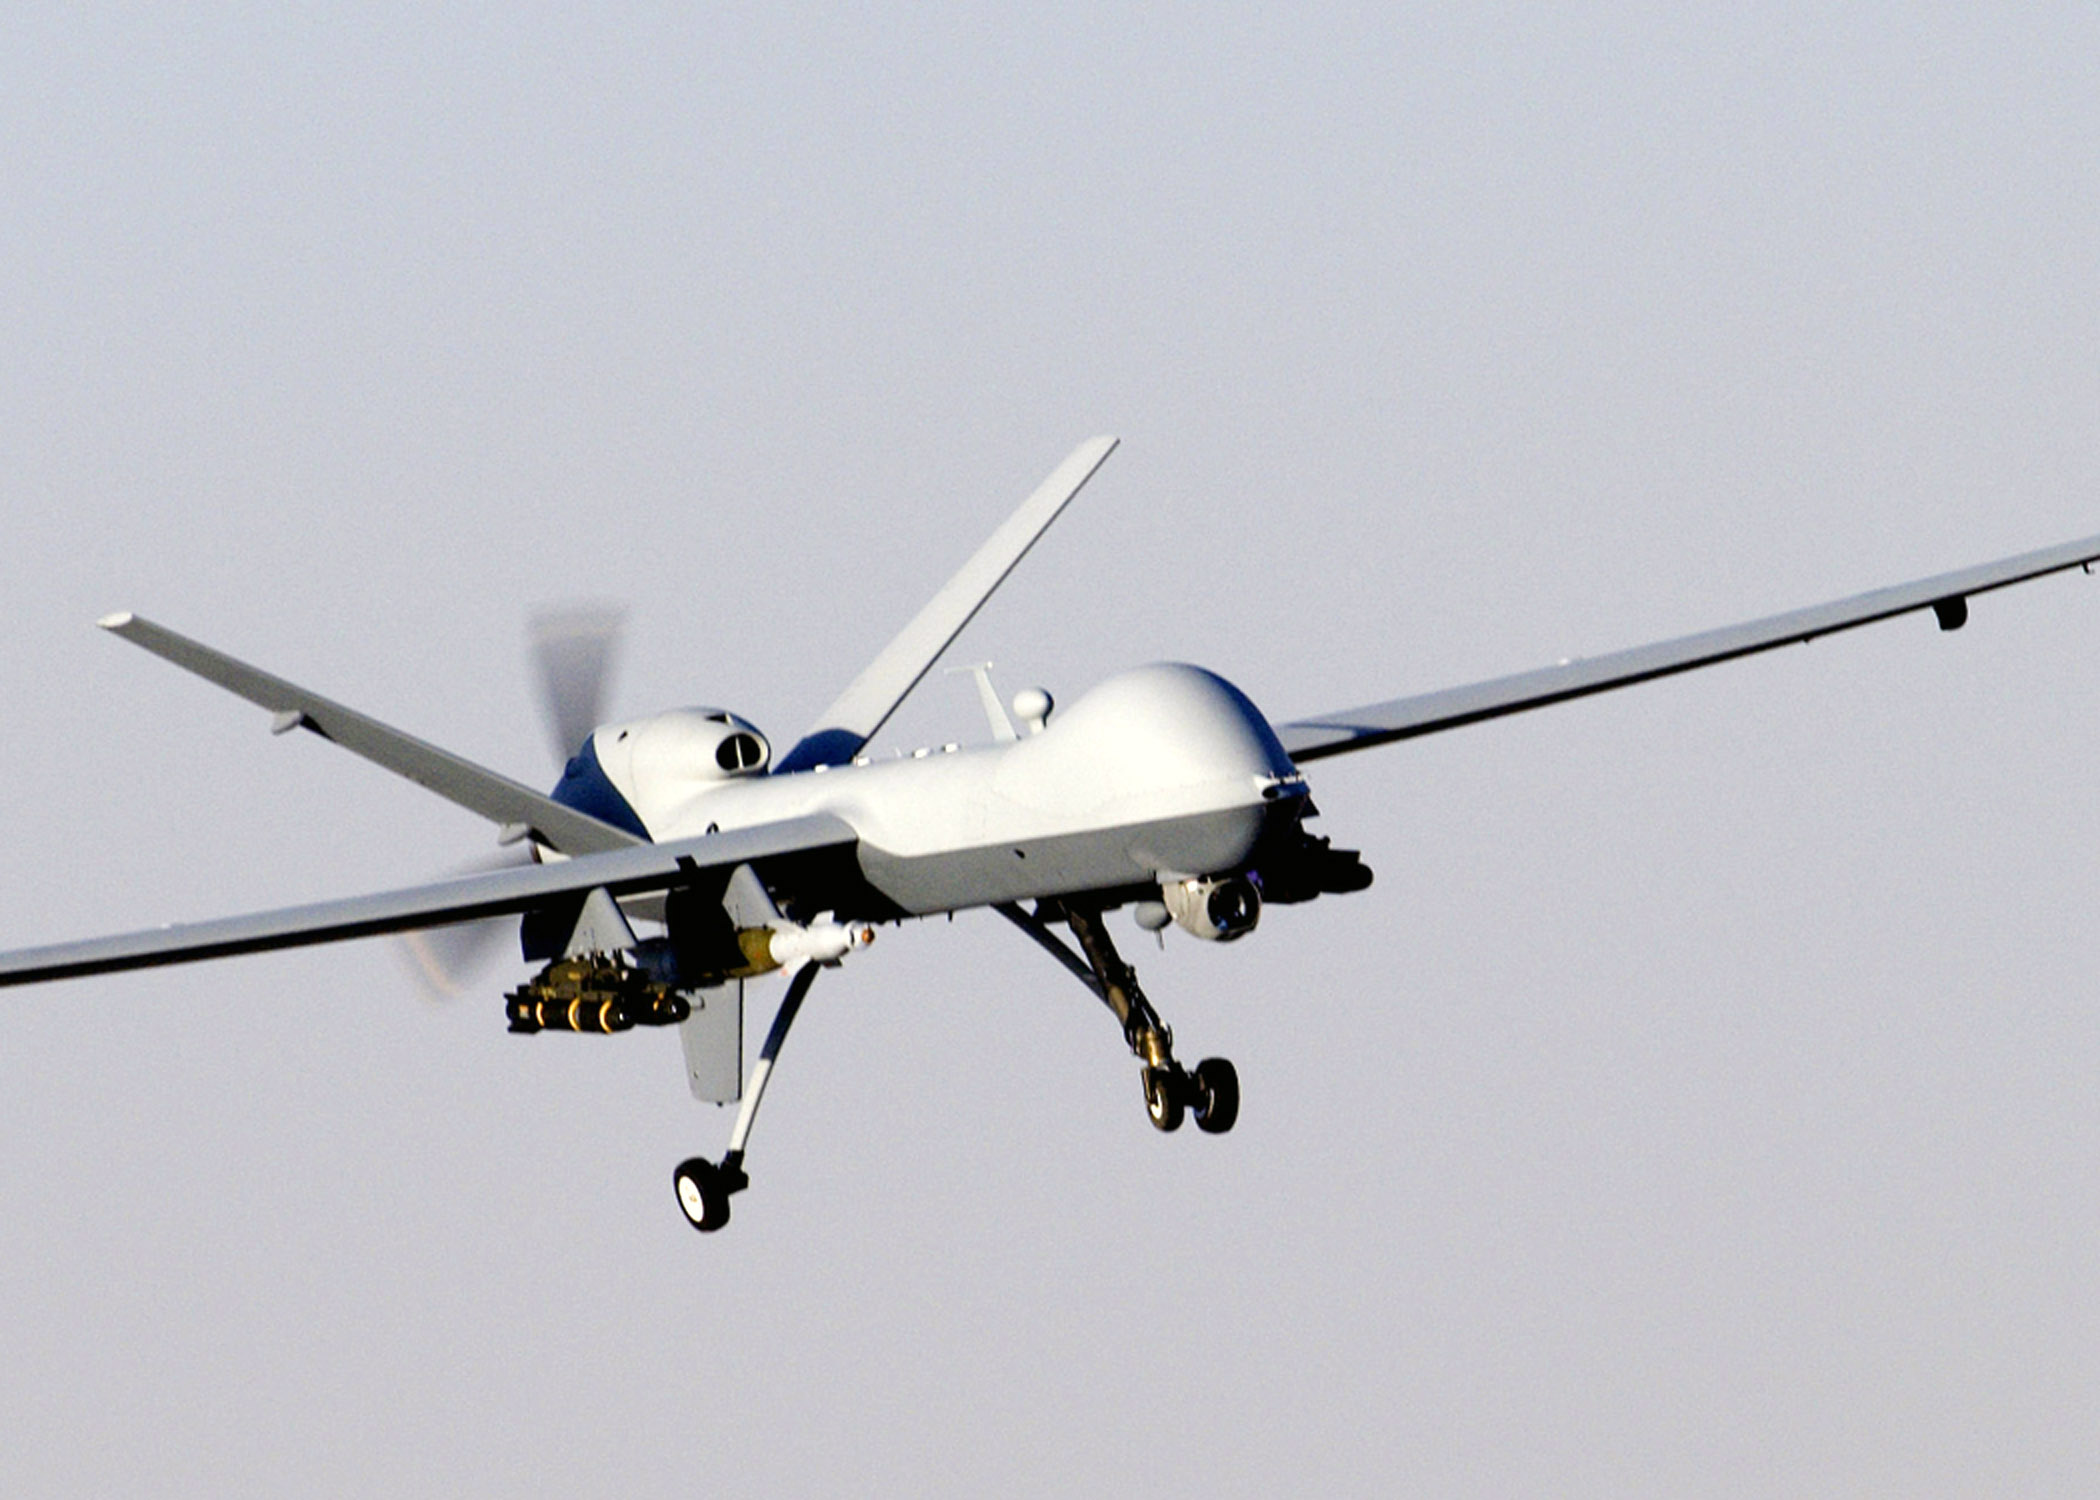
\includegraphics[width=.9\linewidth]{images/UAV.jpg}
  \caption{Unmanned Aerial Vehicle (UAV)}
  \label{fig:sfigUAV}
\end{subfigure} 

\begin{subfigure}{.5\textwidth}
  \centering
  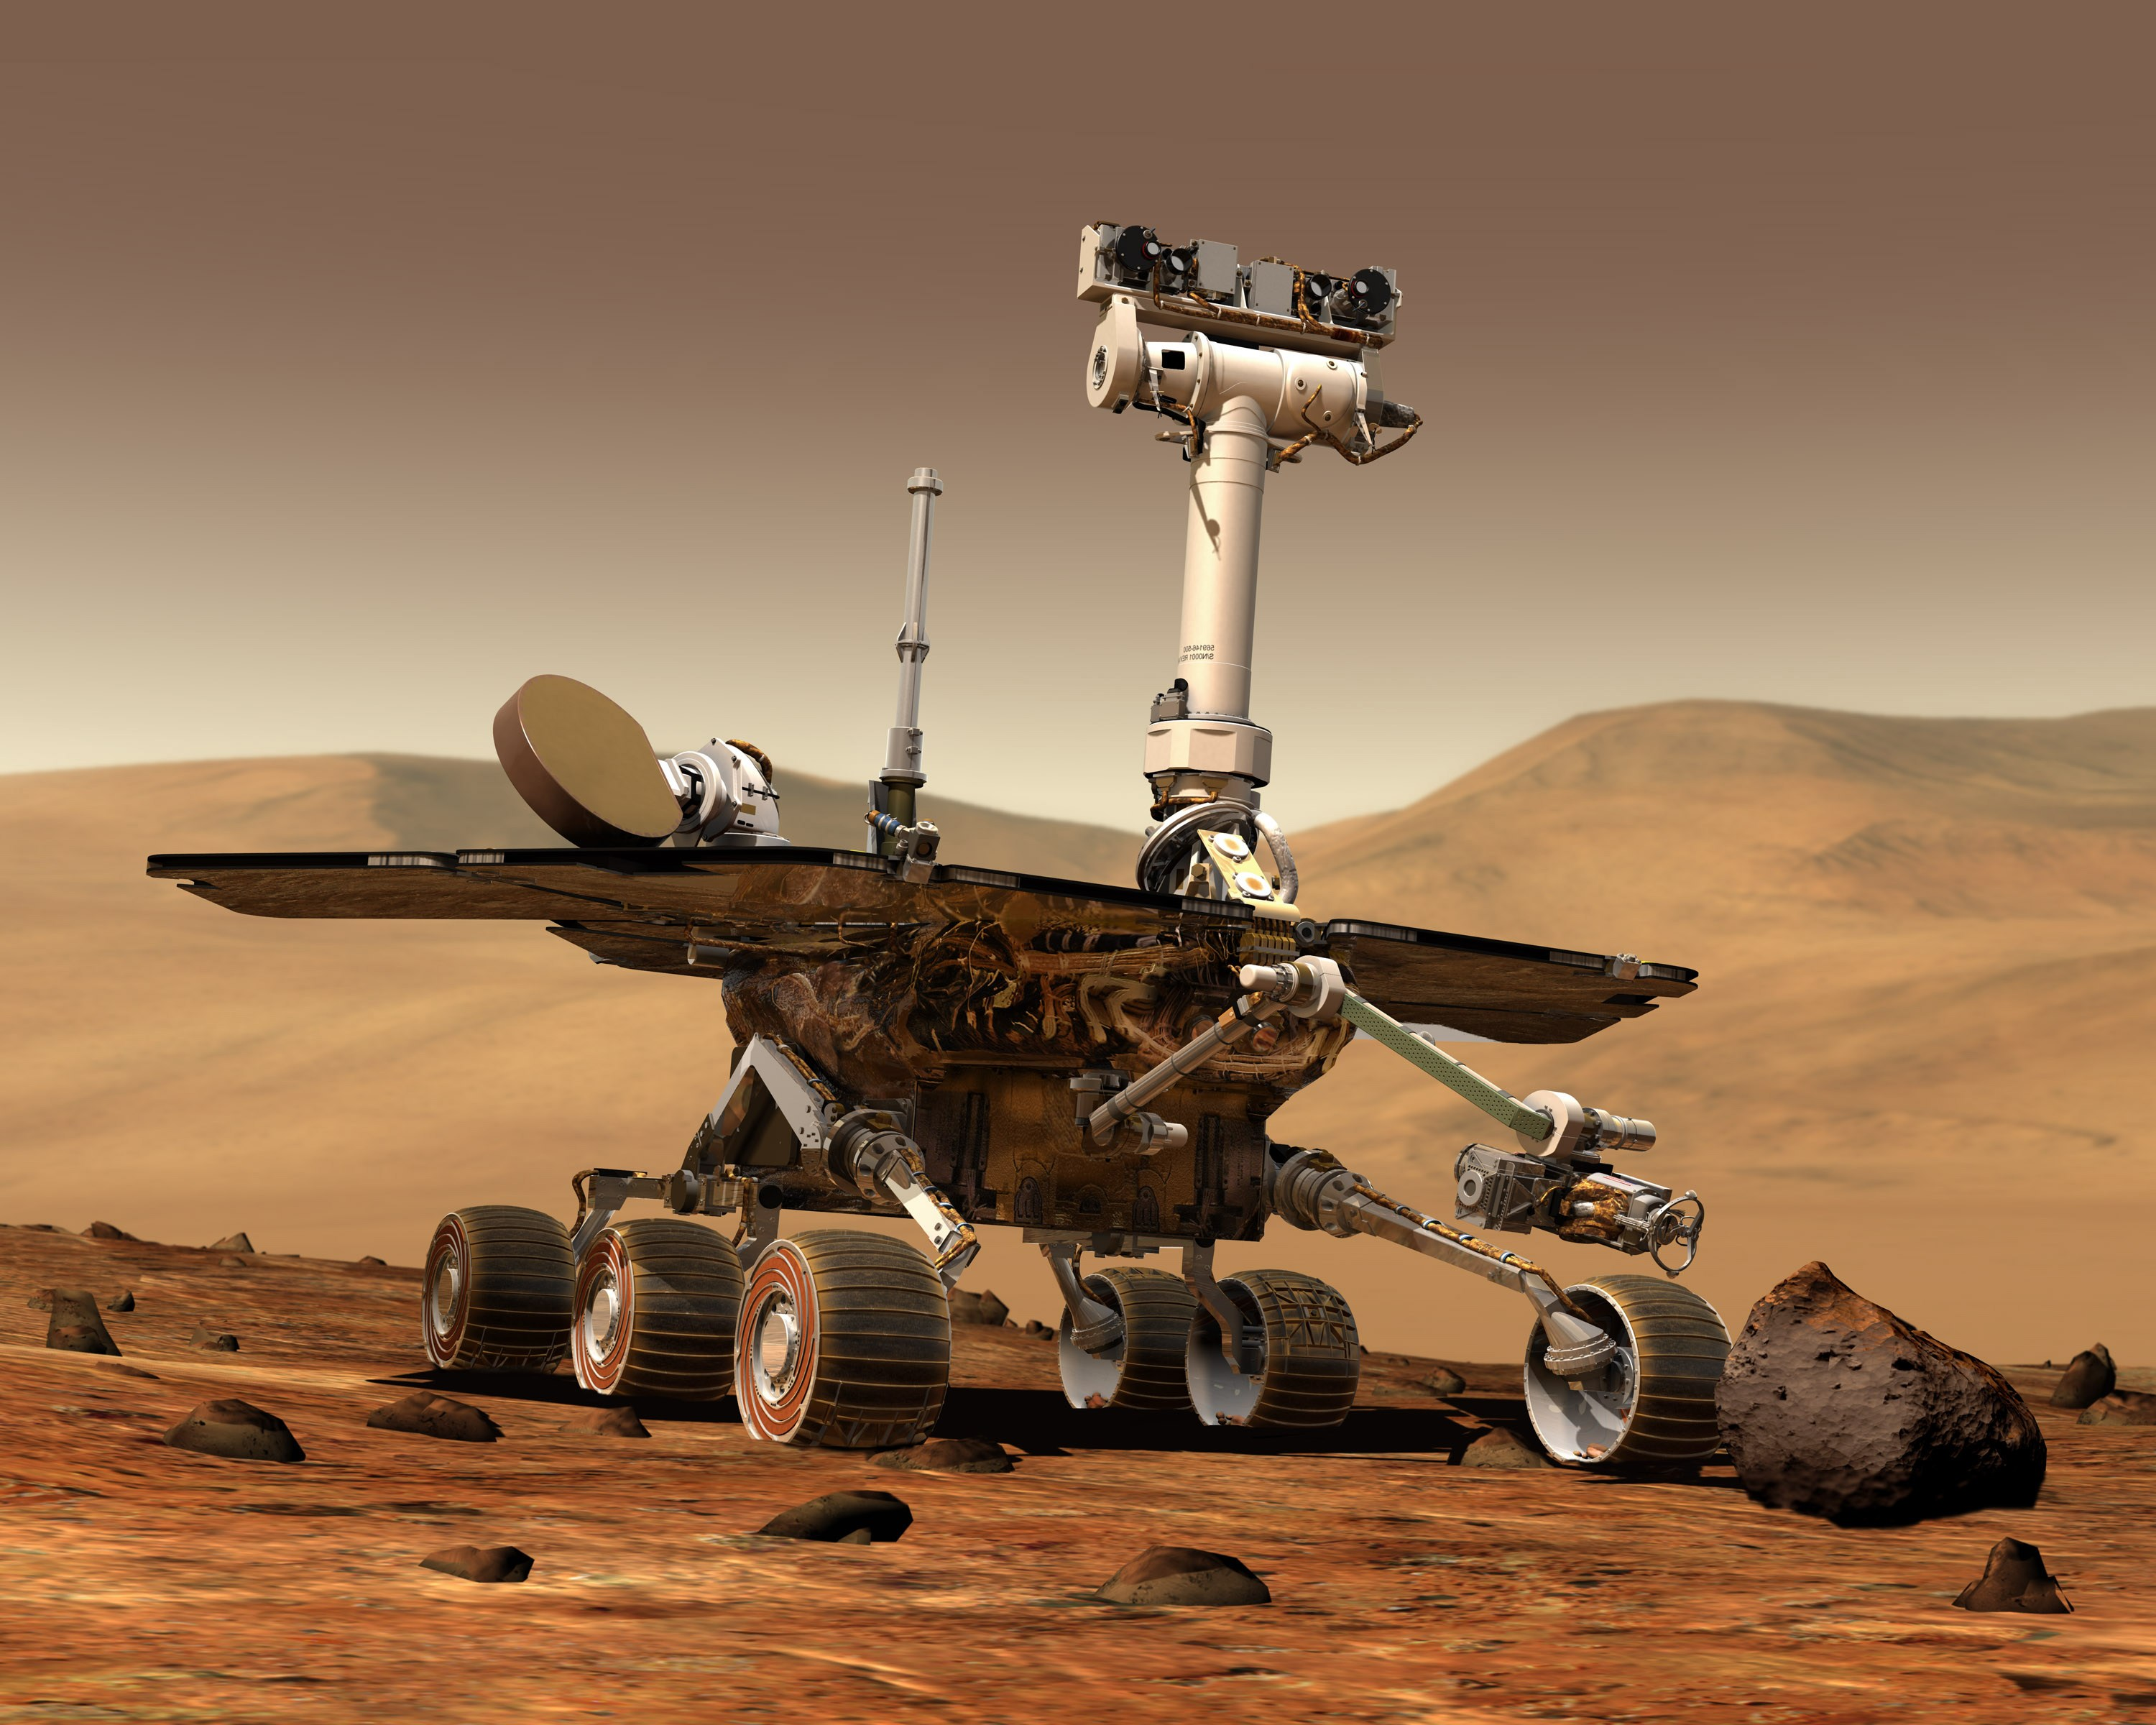
\includegraphics[width=.9\linewidth]{images/ROVER.jpg}
  \caption{Mars Rover}
  \label{fig:sfigROVER}
\end{subfigure} %
\begin{subfigure}{.5\textwidth}
  \centering
  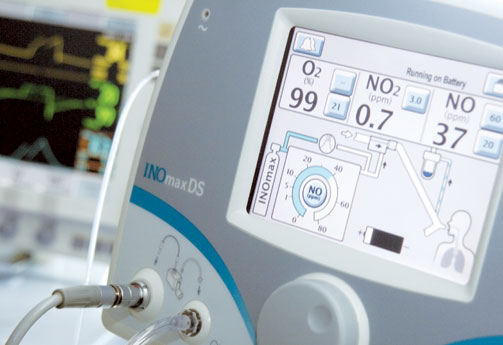
\includegraphics[width= 0.9\linewidth]{images/LSS.jpg}
  \caption{Life Support System}
  \label{fig:sfigLSS}
\end{subfigure} 

\caption{Several Realtime Critical Applications}
\label{fig:fig}
\end{figure}

Notable examples are air traffic control, auto pilot, life support system, smart
power grids, telephone networks, robots like UAV and rovers deployed for
surveillance, reconnaissance and knowledge acquisition in remote locations etc.
These applications are real-time sensitive and there is no room for exception
handling in such system.
Sudden crash involves risk of human life, expensive equipments and critical
services.
Other example includes web applications which uses scrips to dynamically
generate websites and interfaces as per customer preferences.
Many E-commerce websites handles queries, access and process customer and
shopping items data and commits large amount of transactions.
Sudden system crash may result in loss of precious time and data which
eventually may result in a frustrated customers move to other websites.
Many time bad or malicious code leads to some vulnerability to critical
applications and website which can be exploited by attack to orchestrate system
crash. Thought these examples cover a large variety of applications, all of them
point to some concern of \emph{availability}.

Usually, developers tests their code in series of verifications which involves
code review, static and dynamic analysis of the code, generate test cases to
cover as much potential input .Yet may corner cases can be left overlooked which
can cause runtime exceptions.

Multi-threaded applications are also susceptible to erroneous thread
interleaving. One such exception is
\emph{java.lang.IllegalMonitorStateException}, when a thread has attempted to
wait on an object's monitor or to notify other threads waiting on an object's
monitor without owning the specified monitor. Applications under adversarial
situation should be considered where deliberate malicious input may cause it to
fail. To recover from such situation, a mechanism is needed which can predict
failure by doing invariant and symbolic analysis. Invariant analysis will detect
particular variables outside legal/safe bound. Static analysis will indicate
to the potential point of failure.


In this paper we proposed two solution to suppress runtime example and ensure
system survivability. The approach consists of four primary phases

\begin{itemize}
  \item \textbf{Taint Analysis} : We performed static taint analysis to mark all
  the program paths which lead to some tainted sink. The taint analysis goes
  like the following : we marked such variables and objects which are coming
  from outside world (like user input from web page or console), then we looked
  for taint propagating methods by which the tainting can be propagated to some no
  tainted variable or objects from some tainted ones. Then we also enlisted some
  taint sink such as console out put or database commit, which indicates that
  certain tainted variables or objects leaves the system. We marked such paths
  and such statement which involved tainted variables/objects as patching on
  such variables is not recommended.
  \item \textbf{Generate input data-set} : We index user input along with the
  global variables and method arguments of successful runs.
  The local variables are not indexed as they can be re-generated.
  These data-set is used as a reference to later executions which encounters
  runtime exceptions.
  Appropriate user input of previous successful run is chosen in terms of
  correlation coefficient.
  
  \item \textbf{Program slice for patching} : We perform static analysis prior
  to running the program to determine data dependencies of the variables.
  The analysis yields a dependency graph which is used to determine optimal
  slice to be used as patch.
  This patch is placed in catch block and executed with the values of previous
  successful run while the original code is wrapped in try block.
  
  \item \textbf{Determine type of exception and patching} : The characteristics
  of patching is dependent on the type of runtime exception encountered by the
  program. A piece of code may throws multiple types of exceptions and all of
  them are handled at the time of patching by instrumenting multiple catch
  blocks.
  
  \item \textbf{Use typestate for repairing} : Typestate analysis, sometimes
  called protocol analysis defines valid sequences of operations that can be
  typically modeled using Finite State Machine (FSM) where the states represent
  abstract state of the program and the symbols are certain method invocations
  to perform state transition. Typestates are capable of representing behavioral
  type refinements like Iterators, where \emph{hasNext()} method should be
  called before the \emph{next()} method call.
  Typestate analysis is widely used as a safety feature to ensure a certain
  sequence of operations maintains proper protocol or not.
  % But this method is unconventional and investigated in the field of program
  % repairing.
  The documentations of the API used in the application will define the valid
  typestate for repairing.
\end{itemize}

The object of the patching is to repair the problem closest to it to minimize
any collateral damage to other parts of the applications hence minimizing the
chance of unintentional data loss/corruption.




